\documentclass{beamer}
\usepackage{listings}
\lstset
{
language=C,
frame=single, 
breaklines=true,
columns=fullflexible
}
\usepackage{subcaption}
\usepackage{url}
\usepackage{tikz}
\usepackage{graphicx}
\usepackage{multicol}
\usepackage{tkz-euclide} % loads  TikZ and tkz-base
%\usetkzobj{all}
\usetikzlibrary{calc,math}
\usepackage{float}
\usepackage{amsthm}
\newcommand\norm[1]{\left\lVert#1\right\rVert}
\renewcommand{\vec}[1]{\mathbf{#1}}
\newcommand{\R}{\mathbb{R}}
\newcommand{\C}{\mathbb{C}}
\newcommand{\comb}[2]{{}^{#1}\mathrm{C}_{#2}}
\providecommand{\brak}[1]{\ensuremath{\left(#1\right)}}
\providecommand{\abs}[1]{\vert#1\vert}
\providecommand{\fourier}{\overset{\mathcal{F}}{ \rightleftharpoons}}
\providecommand{\sbrak}[1]{\ensuremath{{}\left[#1\right]}}
\usepackage[export]{adjustbox}
\usepackage[utf8]{inputenc}
\usepackage{amsmath}
\usepackage[version=4]{mhchem}
\usetheme{Boadilla}
\title{GATE 2021 (ST), Q.15}
\author{V Rahul}
\institute{IITH}
\date{\today}

\begin{document}

\begin{frame}
  \titlepage
\end{frame}

\begin{frame}{Question}
    \begin{block}{GATE 2021 (ST), Q.15}
        A fair die is rolled twice independently. Let X and Y denote the outcomes of the first and second roll, respectively. Then $E(X+Y\:|\:(X-Y)^2=1)$ equals
    \end{block}
\end{frame}

\begin{frame}{PDF of X+Y}
    PDF of sum of random variables X and Y given their individual PDFs can be calculated using
    \begin{enumerate}
        \item Convolution
        \item Characteristic Function
    \end{enumerate}
\end{frame}

\begin{frame}{PDF of X and Y}
    X and Y are two independent random variables that can take the values 1, 2, 3, 4, 5, 6.
    \begin{align}
        \Pr\brak{X=k}=\frac{1}{6}, 1\leq k \leq 6\\
        \Pr\brak{Y=k}=\frac{1}{6}, 1\leq k \leq 6
    \end{align}
\end{frame}

\begin{frame}{Convolution}
    \begin{block}{}
        The general formula for the distribution of the sum Z=X+Y of two discrete random variables is\\
        \begin{align}
            \Pr\brak{Z=z} = \sum_{k=-\infty}^{\infty} \Pr\brak{X=k,Y=z-k}
        \end{align}
        If X and Y are independent\\
        \begin{align}
            \Pr\brak{Z=z} = \sum_{k=-\infty}^{\infty} \Pr\brak{X=k}\times\Pr\brak{Y=z-k}
        \end{align}
    \end{block}
\end{frame}

\begin{frame}{PDF of X+Y using convolution}
    \begin{block}{}
        $\Pr\brak{X+Y=n}$
        \begin{align}
            =&\sum_{k=n-6}^{n-1} \Pr\brak{X=k}\times\Pr\brak{Y=n-k}, 1\leq k \leq 6\\
            %=&\sum_{k=n-6}^{n-1} \frac{1}{6}\times\frac{1}{6}, 1\leq k \leq 6\\
            =&\sum_{k=n-6}^{n-1} \frac{1}{36}, 1\leq k \leq 6\label{0.0.12}\\
            =&
            \left\{
	        \begin{array}{ll}
		        \frac{n-1}{36}  & ,\: 2 \leq n \leq 7 \\
		        \frac{13-n}{36} & ,\: 8 \leq n \leq 12
	        \end{array}
            \right.
        \end{align}
    \end{block}
\end{frame}

\begin{frame}{PDF of X+Y using convolution}
    \begin{figure}[htb]
        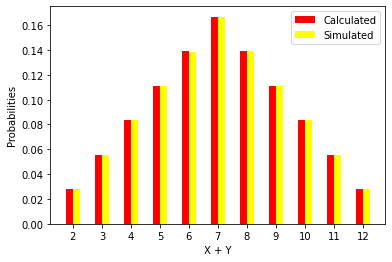
\includegraphics[width=\columnwidth]{Assignment-4(1).png}
        \caption{Plot of PMF for X+Y}
    \end{figure}
\end{frame}

\begin{frame}{PDF of X-Y using convolution}
    \begin{block}{}
        $\Pr\brak{X-Y=n}$
        \begin{align}
            =&\sum_{k=n+1}^{n+6} \Pr\brak{X=k}\times\Pr\brak{Y=k-n}, 1\leq k \leq 6\\
            %=&\sum_{k=n+1}^{n+6} \frac{1}{6}\times\frac{1}{6}, 1\leq k \leq 6\\
            =&\sum_{k=n+1}^{n+6} \frac{1}{36}, 1\leq k \leq 6\label{0.0.16}\\
            =&
            \left\{
	        \begin{array}{ll}
		        \frac{n+6}{36} & ,\: -5 \leq n \leq 0 \\
		        \frac{6-n}{36} & ,\: 1  \leq n \leq 5
	        \end{array}
            \right.
        \end{align}
    \end{block}
\end{frame}

\begin{frame}{PDF of X-Y using convolution}
    \begin{figure}[htb]
        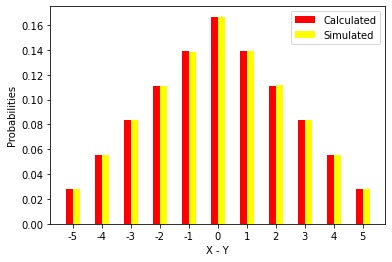
\includegraphics[width=\columnwidth]{Assignment-4(2).png}
        \caption{Plot of PMF for X-Y}
    \end{figure}
\end{frame}

\begin{frame}{Expectation value}
    \begin{block}
        \begin{align}
            E\brak{X}=\sum x_{i}\times\Pr\brak{X=x_{i}}\\
            \Pr\brak{A|B}=\frac{\Pr\brak{A,B}}{{B}}
        \end{align}
        $E\brak{X+Y\:|\:(X-Y)^2=1}$
        \begin{align}
            =&\sum\:n\times\Pr\brak{X+Y=n\:|\:(X-Y)^2=1}\\
            =&\sum\:n\times\frac{\Pr\brak{X+Y=n,(X-Y)^2=1}}{\Pr\brak{(X-Y)^2=1}}
        \end{align}
    \end{block}
\end{frame}

\begin{frame}{Solution contd.}
    \begin{align}
        \begin{split}
            =\sum\:n\times\frac{\Pr\brak{X+Y=n,(X-Y)=1}}{\Pr\brak{(X-Y)=1}}
            \bigskip\\
            \times\Pr\brak{(X-Y)=1|(X-Y)^2=1}
            \bigskip\\
            +\sum\:n\times\frac{\Pr\brak{X+Y=n,(X-Y)=-1}}{\Pr\brak{(X-Y)=-1}}
            \bigskip\\
            \times\Pr\brak{(X-Y)=1\:|\:(X-Y)^2=1}
        \end{split}
    \end{align}
    \begin{align}
        \begin{split}
            =\:\frac{\Pr\brak{(X-Y)=1\:|\:(X-Y)^2=1}}{\Pr\brak{(X-Y)=1}}
            \bigskip\\
            \times\sum\:n\times\Pr\brak{X+Y=n,(X-Y)=1}
            \bigskip\\
            +\frac{\Pr\brak{(X-Y)=-1\:|\:(X-Y)^2=1}}{\Pr\brak{(X-Y)=-1}}
            \bigskip\\
            \times\sum\:n\times\Pr\brak{X+Y=n,(X-Y)=-1}\label{0.0.8}
        \end{split}
    \end{align}
\end{frame}

\begin{frame}{Solution contd.}
    Using equations \eqref{0.0.12} and \eqref{0.0.16} in \eqref{0.0.8}\\
    We get,\\
    \newline
    $E\brak{X+Y\:|\:(X-Y)^2=1}$
    \begin{align}
        =&\:\brak{\frac{\frac{1}{2}}{\frac{5}{36}}}\times\brak{\frac{35}{36}}+\brak{\frac{\frac{1}{2}}{\frac{5}{36}}}\times\brak{\frac{35}{36}}\\
        =&\:7
    \end{align}
\end{frame}

\begin{frame}{Characteristic Function}
  \begin{enumerate}
    \item If a random variable admits a probability density function, then the characteristic function
          is the Fourier transform of the probability density function.
    \item    It provides an alteranate way to deal with probabilities of random variables
          other than PDF and CDF.
    \item It has particularly simpler results in case of sum of independent random varaiables.
  \end{enumerate}
\end{frame}
\begin{frame}{PDF of X+Y using characteristic function}
  \begin{block}{Property}
    Characteristic function of sum of independent random variables is the product of characteristic function of those random varaiables.
  \end{block}
  And we obtain the PDF of X+Y by calculating the inverse characteristic function of X+Y.
\end{frame}
\begin{frame}{CF of X and Y}
  \begin{block}{Given PDF of X and Y}
    \begin{align}
      f(t) = \displaystyle\frac{1}{\pi} \frac{1}{1+{t}^2} \hspace{0.2cm},-\infty < t < +\infty\label{0.0.1}
    \end{align}
  \end{block}
  We then calcultate the fourier transform of $f(t)$ to get the CF of X and Y.
  \begin{block}{CF of X and Y}
    \begin{align}
      g(w) =\hspace{0.2cm} & \int_{-\infty}^{\infty}  f(t) {e}^{iwt} dt                                         \\[0.2cm]
      =\hspace{0.2cm}      & \int_{-\infty}^{\infty}  \displaystyle\frac{1}{\pi} \frac{1}{1+{t}^2} {e}^{iwt} dt \\[0.2cm]
      =\hspace{0.2cm}      & e^{-\abs{w}}\hspace{0.2cm}, -\infty<w<\infty
    \end{align}
  \end{block}
\end{frame}
\begin{frame}{CF-contd.}
  Let CF of Z = X + Y be h(w)
  \begin{block}{h(w)}
    \begin{align}
      h(w) = & \hspace{0.2cm} \text{CF of x $\times$ CF of Y}  \\
      =      & \hspace{0.2cm} e^{-\abs{w}} \times e^{-\abs{w}} \\
      =      & \hspace{0.2cm} {e}^{-2\abs{w}}
    \end{align}
  \end{block}
\end{frame}

\begin{frame}{Inverse CF of Z}
  Now to find the PDF of Z, we calcultate the inverse fourier transform of h(w).
  \begin{block}{Finding $F_{X+Y}(t)$}
    \begin{align}
      F_{X+Y}(t) =\hspace{0.2cm} & \int_{-\infty}^{\infty} h(w) {e}^{-iwt} dw           \\[0.2cm]
      =\hspace{0.2cm}            & \int_{-\infty}^{\infty} {e}^{-iwt-2\abs{w}} dw       \\[0.2cm]
      =\hspace{0.2cm}            & \frac{4}{4 + {t}^2} \hspace{0.2cm}, -\infty<t<\infty
    \end{align}
  \end{block}
\end{frame}
\begin{frame}{Solution contd.}
  \begin{block}{$F_{X+Y}(t)$}
    \begin{align}
      \text{But}\hspace{0.2cm} \int_{-\infty}^{\infty} F_{X+Y}(t) dt = \int_{-\infty}^{\infty} \frac{4}{4+{t^2}} dt= 2\pi
    \end{align}
    So we plug in the normalisation factor $\displaystyle\frac{1}{2\pi}$ and the new $F_{X+Y}$ becomes
    \begin{align}
      F_{X+Y}(t) = \frac{2}{\pi} \frac{1}{4+{t}^2}\hspace{0.2cm}, -\infty<t<\infty
    \end{align}
  \end{block}
\end{frame}
\begin{frame}{Fun Approach}
  \begin{block}{Recap}
    \begin{align}
      g(w) = & \hspace{0.2cm}  \int_{-\infty}^{\infty}  f(t) {e}^{iwt} dt     \label{0.0.13} \\
      =      & \hspace{0.2cm}  e^{-\abs{w}}\hspace{0.2cm}, -\infty<w<\infty                  \\
      h(w) = & \hspace{0.2cm} {e}^{-2\abs{w}}\hspace{0.2cm}, -\infty<w<\infty
    \end{align}
  \end{block}
  Notice that $g(2w) = h(w)$\\
  Fourier transform obeys one to one correspondence
\end{frame}
\begin{frame}{Solution contd.}
  Replacing $w$ with $2w$ in \eqref{0.0.13}
  \begin{block}{$g(2w)$}
    \begin{align}
      g(2w) = & \hspace{0.2cm}  \int_{-\infty}^{\infty}  f(t) {e}^{i(2w)t} dt                                         \\
      =       & \hspace{0.2cm}  \int_{-\infty}^{\infty}  f\brak{\frac{t}{2}} {e}^{i2w\frac{t}{2}} d\brak{\frac{t}{2}} \\
      =       & \hspace{0.2cm}  \int_{-\infty}^{\infty}  \frac{1}{2} f\brak{\frac{t}{2}} {e}^{iwt} dt
    \end{align}
  \end{block}
\end{frame}
\begin{frame}{Solution contd.}
  Since $g(2w) = h(w)$
  \begin{block}{$h(w)$}
    \begin{align}
      h(w) = & \hspace{0.2cm}  \int_{-\infty}^{\infty}  \frac{1}{2} f\brak{\frac{t}{2}} {e}^{iwt} dt
    \end{align}
  \end{block}
  Let $\frac{1}{2} f\brak{\frac{t}{2}}$ be any function of t whose Characteristic function is h(w).
\end{frame}
\begin{frame}{Solution contd.}
  Recall from $\eqref{0.0.1}$ f(t) = $\displaystyle\frac{1}{\pi} \frac{1}{1+{t}^2} \hspace{0.2cm},-\infty < t < +\infty$
  \begin{block}{}
    \begin{align}
      F_Z(t) = & \hspace{0.2cm} \frac{1}{2} f\brak{\frac{t}{2}}                                                 \\
      =        & \hspace{0.2cm} \frac{1}{2} \displaystyle\frac{1}{\pi}  \frac{4}{4+{t}^2}                       \\
      =        & \hspace{0.2cm} \displaystyle\frac{1}{\pi}  \frac{2}{4+{t}^2} \hspace{0.2cm}, -\infty<t<+\infty
    \end{align}
  \end{block}
\end{frame}

\begin{frame}{$\frac{Z}{3} = \frac{X+Y}{3}$}
  We know that if a random variable M has a probability density $f_M(x)$, then the probability density of random variable kM is
  \begin{block}{}
    \begin{align}
      f_{kM}\brak{x} = \frac{1}{\abs{k}} f_M\brak{\frac{x}{\abs{k}}}
    \end{align}
  \end{block}
  Probability density of $\frac{Z}{3}$ given $F_Z(t)$ is
  \begin{block}{}
    \begin{align}
      F_{\frac{Z}{3}}(t) = & 3\times \displaystyle f_{X+Y}(3t)                                 \\
      =                    & \frac{6}{\pi} \frac{1}{4+9{t}^2}\hspace{0.2cm}, -\infty<t<+\infty
    \end{align}
    \begin{center}
      Thus option 1 is correct
    \end{center}
  \end{block}
\end{frame}
\begin{frame}{Figures}
  \begin{figure}[!]
    \centering
     \includegraphics[width = 0.8\columnwidth]{Presentation-1.png}
    \caption{PDF of X,Y and $\displaystyle\frac{X+Y}{3}$}
  \end{figure}
\end{frame}
\end{document}